\hthree{Implementierung}

\sectionauthor{Julian Kusternigg}

\hfour{Einleitung}

Wie der Rest von ZELIA ist auch der Code im Frontend in Typescript geschrieben, um einen Überblick über die Datentypen zu behalten. Zusätzlich bringt es noch Vorteile bei der Implementierung des Komponentensystems. Wie schon gesagt ist das Komponentensystem, neben dem Client-Side-Router, der zweite Teil unserer Frontend Bibliothek, den wir selbst entworfen haben, um unsere Webseite darstellen zu können. Somit müssen wir uns nicht auf andere Frameworks verlassen, die in den meisten Fällen nicht so performant sind, da unsere Bibliothek perfekt an die Bedürfnisse von ZELIA angepasst ist.

\hfour{Architektur}

Wie eben im Standard beschrieben muss es eine Klasse geben, welche von "HTMLElement" erbt, um als "Custom HTML Element" verwendet werden zu können. So gibt es in der ZELIA Implementierung die abstrakte Klasse "Component" von der alle anderen Komponenten erben.

\typescript{code/WebComponents/BaseInterfaces.ts}{Schnittstellen der Basiskomponente}

Die jeweils dazugehörige HTML Quelle wird vom sogenannten "Component Loader", beim Aufruf der Webseite, geladen und zwischengespeichert. Dadurch muss nicht jede Komponente ihren Darstellungscode selbst herunterladen, wenn sie verwendet wird, wie es bei manchen Bibliotheken sonst der Fall ist. Somit ist es kaum merkbar, wenn man eine Seite wechselt, denn die Seite kann schon angezeigt werden, während die nötigen Infos noch nachgeladen werden.

Mit Hilfe von "States" kann man Text dynamisch ersetzen, wie es auch in anderen Bibliotheken gemacht wird.

\html{code/WebComponents/State.html}{Ersetzungsmechanismus (HTML)}

\typescript{code/WebComponents/State.ts}{Ersetzungsmechanismus (Javascript)}

Dadurch können zum Beispiel nachgeladene Daten eingefügt werden, aber auch die Sprache der Seite kann so geändert werden.

Zusätzlich kann sich das Komponentensystem automatisch Referenzen auf "HTML Elemente" suchen. Dafür muss im Konstruktor von der Basiskomponente, von der alle Komponenten erben, nur definiert sein, wie ein Element gefunden wird. Um die Richtigkeit der Datentypen und die automatische Vervollständigung aufrecht zu erhalten, wird als generischen Typ der Komponente mitgegeben welche Datentypen die Elemente haben, die automatisch gefunden werden.

\typescript{code/WebComponents/AutoRef.ts}{Erstellen einer Komponente und suchen einer Referenz}

In diesem Beispiel wird das Element "button" gesucht. Dieses Element ist vom Typ "HTMLButtonElement" und kann mit "\#btnInfo" gefunden werden. Die Raute im Suchfeld besagt, dass der nachfolgende Text die ID von dem HTML-Element ist. Somit würde der Suchtext für das folgende Beispiel zutreffen:

\html{code/WebComponents/IDButton.html}{Beispiel eines HTML Knopfes mit ID}

Im Endeffekt steht dann auf dem Knopf "Click Me". Das "Click" wird mithilfe der
"States" ersetzt und danach wird über die Elementreferenz ein " Me" angehängt. Das automatische Finden von Referenzen ist wichtig, um Events abzufangen oder Elemente zu modifizieren, wenn es notwendig ist.

Wie oben kurz erwähnt, lädt der "Component Loader" die notwendigen HTML-Files und speichert sie. Verwendet werden die Daten dann von der Basis "Component" Klasse, welche im Konstruktor einen Parameter bekommt, in dem der Name des HTML Elements steht. Über diesen Namen holt sich die Komponente, wenn sie erstellt wird, die HTML Ressource. Wenn sie schließlich angezeigt werden soll, ersetzt sie die "States" und fügt sich selbst in die Webseite hinzu.

\typescript{code/WebComponents/ComponentLoader.ts}{Laden einer Komponente}

Erst nachdem alle Ressourcen der Komponenten geladen wurden, wird der Client-Side-Router (siehe Kapitel Client-Side-Router) erstellt und somit die Seite gestartet. Dadurch kann sichergestellt werden, dass keine verzögerten Ladezeiten durch das Laden der Ressourcen auftreten.

\hfour{"Life-Cycle"}

Wenn nun ein eigenes Element erstellt wird, hat der "Loader" die HTML-Ressource, falls es eine gibt, bereits geladen. Während der Initialisierung des Elements, holt sich dieser die HTML-Ressource als Text. Im Konstruktor der Basiskomponente gibt es neben dem "query"-Parameter, welcher für die automatische Referenzierung verwendet wird, noch die "autoRender" und "useShaddowRoot" Argumente. Standardmäßig sind beide Werte auf Wahr gesetzt. Das heißt die Komponente wird, sobald sie auf die Seite hinzugefügt wird, ihr HTML anzeigen und in ein "ShadowRoot" eingebunden werden. Durch das "ShadowRoot" wird es als eigenes Dokument angezeigt, unabhängig von dem wo es eingebunden wird, was Überschneidungen von verschieden CSS-Styles behebt. Somit sieht die Komponente jedes Mal gleich aus, unabhängig von der restlichen Seite.

Bevor der HTML-Text dargestellt werden kann, werden die States ersetzt. Danach wird geschaut ob die Elemente die automatisch referenziert werden sollen, vorhanden sind. Falls sich ein "State" ändert, wird der Inhalt der Komponente automatisch neu erstellt und gerendert. Durch das neu Erstellen der Komponente bekommen auch die referenzierten Elemente neue Referenzen. Das könnte ein Problem sein, wenn man Komponenten hat bei denen es wichtig ist, dass die Elemente "dieselben" bleiben. Somit sollte man sich um das Modifizieren dieser Komponenten selbst kümmern oder keine States ändern, sodass nicht neu gerendert werden muss.

\hfour{Eingebaute Komponenten}

Insgesamt besteht das komplette Frontend aus 12 Komponenten, die auf 7 Seiten verteilt sind. Zusätzlich gibt es die "Debug"-Komponente, die uns während der Entwicklung einen Logger zu Verfügung gestellt hat, der vor allem praktisch war, um auf Mobilgeräten die Hintergrundaufgaben mitverfolgen zu können.

\hfive{Die Startseite}

Auf dem Root-Pfad ("/") liegt unsere Willkommensseite. Auf ihr findet man die Raum-\\eingabekomponente, die von der ZELIA-API alle möglichen Raumnummern abfragt und als Auswahlhilfe anzeigt. Auf Mobilgeräten, wie Smartphones oder Tablets, wird zusätzlich ein Knopf angezeigt, der es möglich macht, die Raumnummer mit der Kamera des Geräts einzulesen. Wenn man auf diesen Knopf drückt, wird man zur "OCR"-Seite weitergeleitet. Gibt man die Raumnummer selbst ein, so landet man auf der Rauminformationsseite. Während der manuellen Eingabe, werden alle bekannten Räume als "Dropdown" unter der Eingabebox angezeigt. Gibt man die ersten Buchstaben des Raumnamens oder Raumnummer an, so werden nur mehr Ergebnisse angezeigt, die dem angegebenen Muster entsprechen.

Beispiel:

\image{media/WebComponents/Startseite_light}{Startseite}

\hfive{Die "OCR"-Seite}

Auf dieser Seite können alle Geräte, die eine Kamera haben, mittels "Optical Character Recognition" (siehe Kapitel Optical Character Recognition), die Raumnummer abscannen, zum Beispiel von Raumschildern, die vor den Räumen hängen. Aufgebaut ist die Seite mit einer Komponente, welche anzeigt was die Kamera sieht und einer Zweiten die als Link dient, um zurück zur Startseite zu kommen. Die Komponente, welche den Scanner anzeigt, ist auch zuständig um den OCR-Service (Tesseract) zu starten und mit Hilfe von diesem den Text aus den Bildern auszulesen. Bevor das Bild an den OCR-Service übergeht, wird es auf 2 Farben komprimiert und so klein zusammengeschnitten, dass nur mehr der markierte Fokusteil der Kamera weiter zu verabreiten bleibt.

% TODO: Bild von der Seite

Meist liefert der OCR-Prozess gut erkennbare Ergebnisse. Allerdings kann es auch passieren, gerade wenn viele helle und dunkle Flecken im Hintergrund des Bildes sind, dass diese als Zeichen erkannt werden. Somit ist wichtig, dass nachdem das Bild in Text umgewandelt wurde, mittels "Regular Expressions" der wichtige Teil aus dem Text herausgefiltert wird. Dieser gesamte Prozess, der Bilder in Text umwandelt, wird einmal pro Sekunde gemacht. Dieser Wert ist einfach änderbar, aber wir haben uns nach längerem Testen dazu entschieden, dass eine Sekunde völlig ausreichen ist, um schnell Raumnummern zu erfassen. Würde der Wert kleiner werden, also wenn mehrmals pro Sekunde Bild zu Text verarbeitet wird, so würden schwächere Smartphones schnell warm werden und mehr Energie verbrauchen. Mehr zu OCR und unseren Messungen später (siehe Kapitel "Optical Character Recognition"). Wenn eine Raumnummer erfolgreich eingelesen wurde, wird man automatisch auf die Rauminformationsseite weitergeleitet.

\hfive{Rauminformationsseite}

Wie der Name schon vermuten lässt, kann man auf der Rauminformationsseite alle Daten über einen Raum auslesen. Nachdem man einen Raum, entweder duch manuelle Eingabe oder duch das Einscannen der Nummer, ausgewählt hat, wird man auf die jeweilige Rauminformationsseite umgeleitet. Aufgebaut ist die Seite aus insgesamt fünf Komponenten. So wie bei der OCR-Seite gibt es auch hier einen Link, welcher zurück auf die Startseite führt. Zwei weitere Komponenten dienen als Knöpfe um eine Meldung oder Buchung zu einem Raum zu erstellen. Wenn man einen der Beiden drückt, wird man auf die jeweilige Seite, Meldung oder Buchung, umgeleitet. Die letzten zwei Komponenten auf dieser Seite sind die intersantesten, denn sie zeigen die Informationen zu einem Raum an. Die Eine zeigt eine aufklappbare Liste an, um die physikalischen Daten eines Raumes anzusehen. Die andere Komponente wird verwendet um den jeweiligen Raumstundenplan dazustellen.

Beispiel:

\begin{figure}[H]
    \centering
    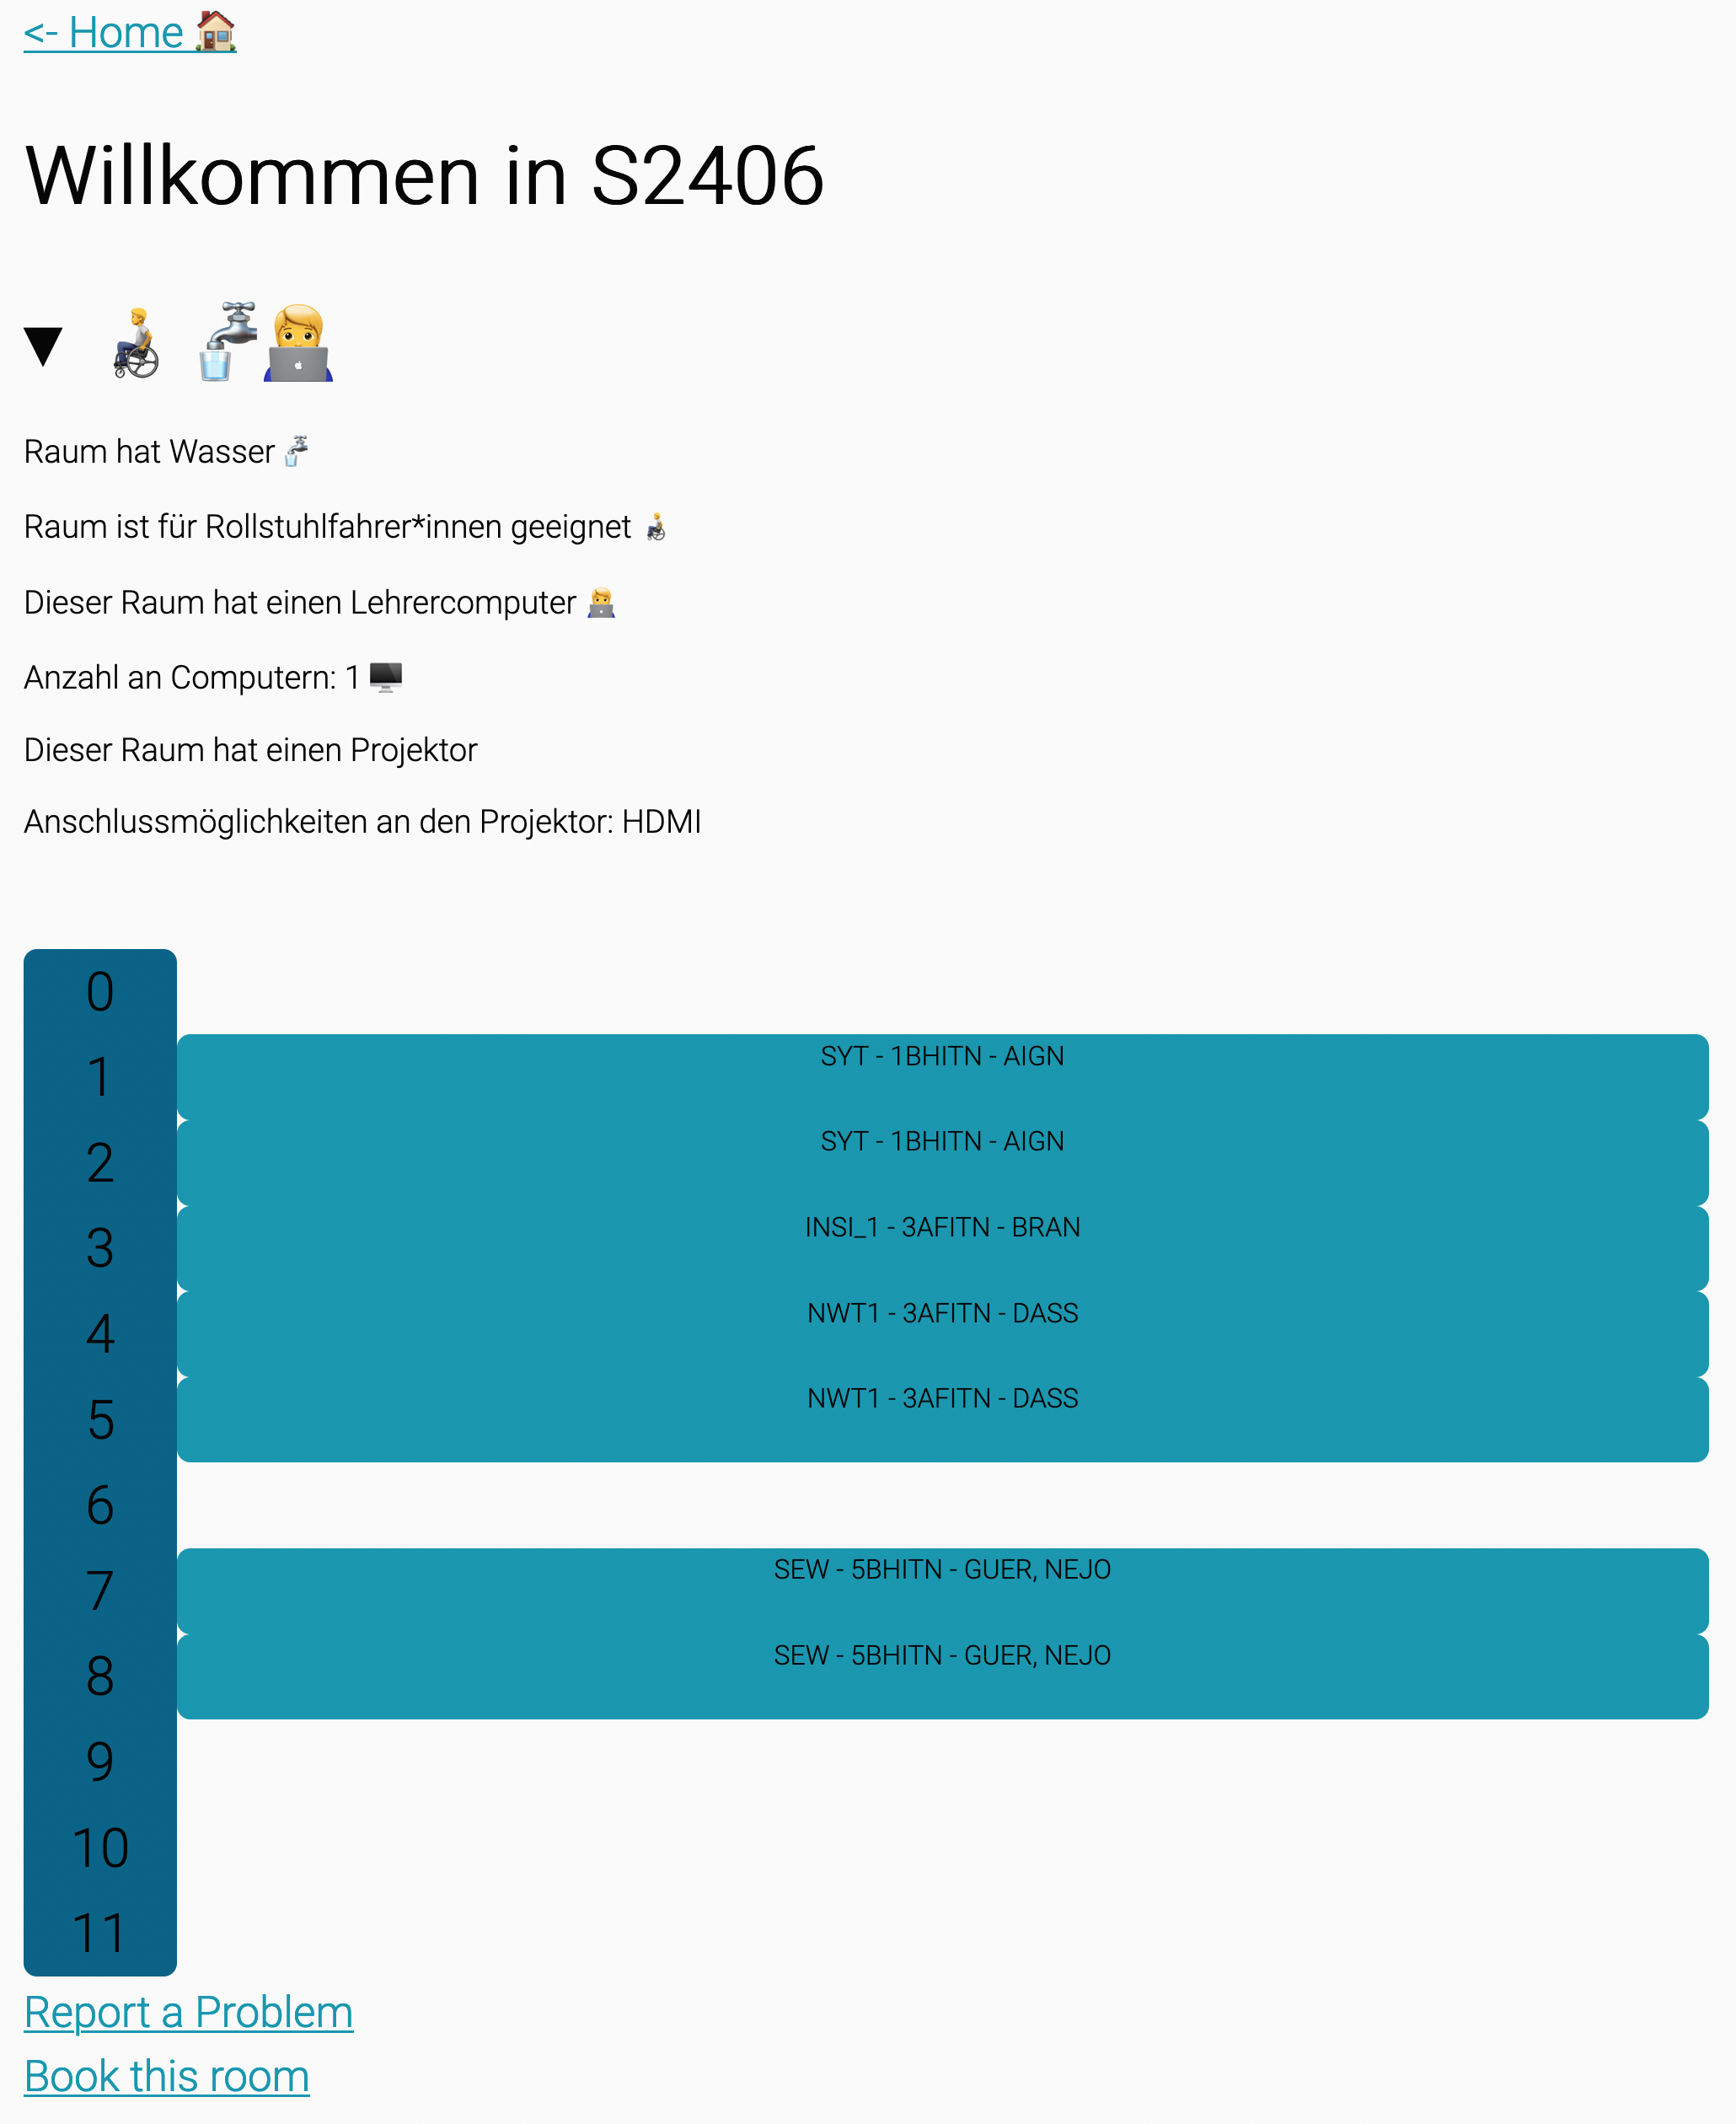
\includegraphics[width=120mm]{media/WebComponents/Rauminformationsseite_light.png}
    \caption{Meldungsseite}
\end{figure}

\hfive{Meldungen und Buchungen}

Die Meldungs und Buchungsseite sind zwei verschiedene Seiten, welche aber recht ähnlich aufgebaut sind. Erreichen kann man sie nur über die Rauminformationsseite, da sie sich auf einen bestimmten Raum beziehen. Dadurch, dass sie zwei verschiedene Aufgaben haben, müssen sie allerdings getrennt behandelt werden und können nicht auf eine Seite zusammengefasst werden. Beide Seiten bestehen aus zwei Komponenten: Einem Formular zur Beischreibung und Angabe der Daten und einem Link, welcher zurück zur Rauminformationsseite führt.
  

Um einen Defekt aus einem Raum zu melden braucht man eine EDU-Mailadresse, das Datum und die Uhzeit wann der Defekt das erste Mal aufgetreten ist und eine Beschreibung um das Problem kurz zu umschreiben. Wie schon erläutert wird die Mailadresse verwendet um Schüler*innen identifiziern zu können, ohne das sie sich selbst einen Account anlegen müssen. Nach Absenden des Formulares bekommt man einen Bestätigungslink auf die angegebene Mailadresse um die Meldung zu bestätigen. Somit ist das Meldesystem nicht anonym da sonst viele Falsch-Meldungen entstehen könnten und trotzdem kann ZELIA angehm ohne Account verwendet werden. 

\begin{figure}[H]
    \centering
    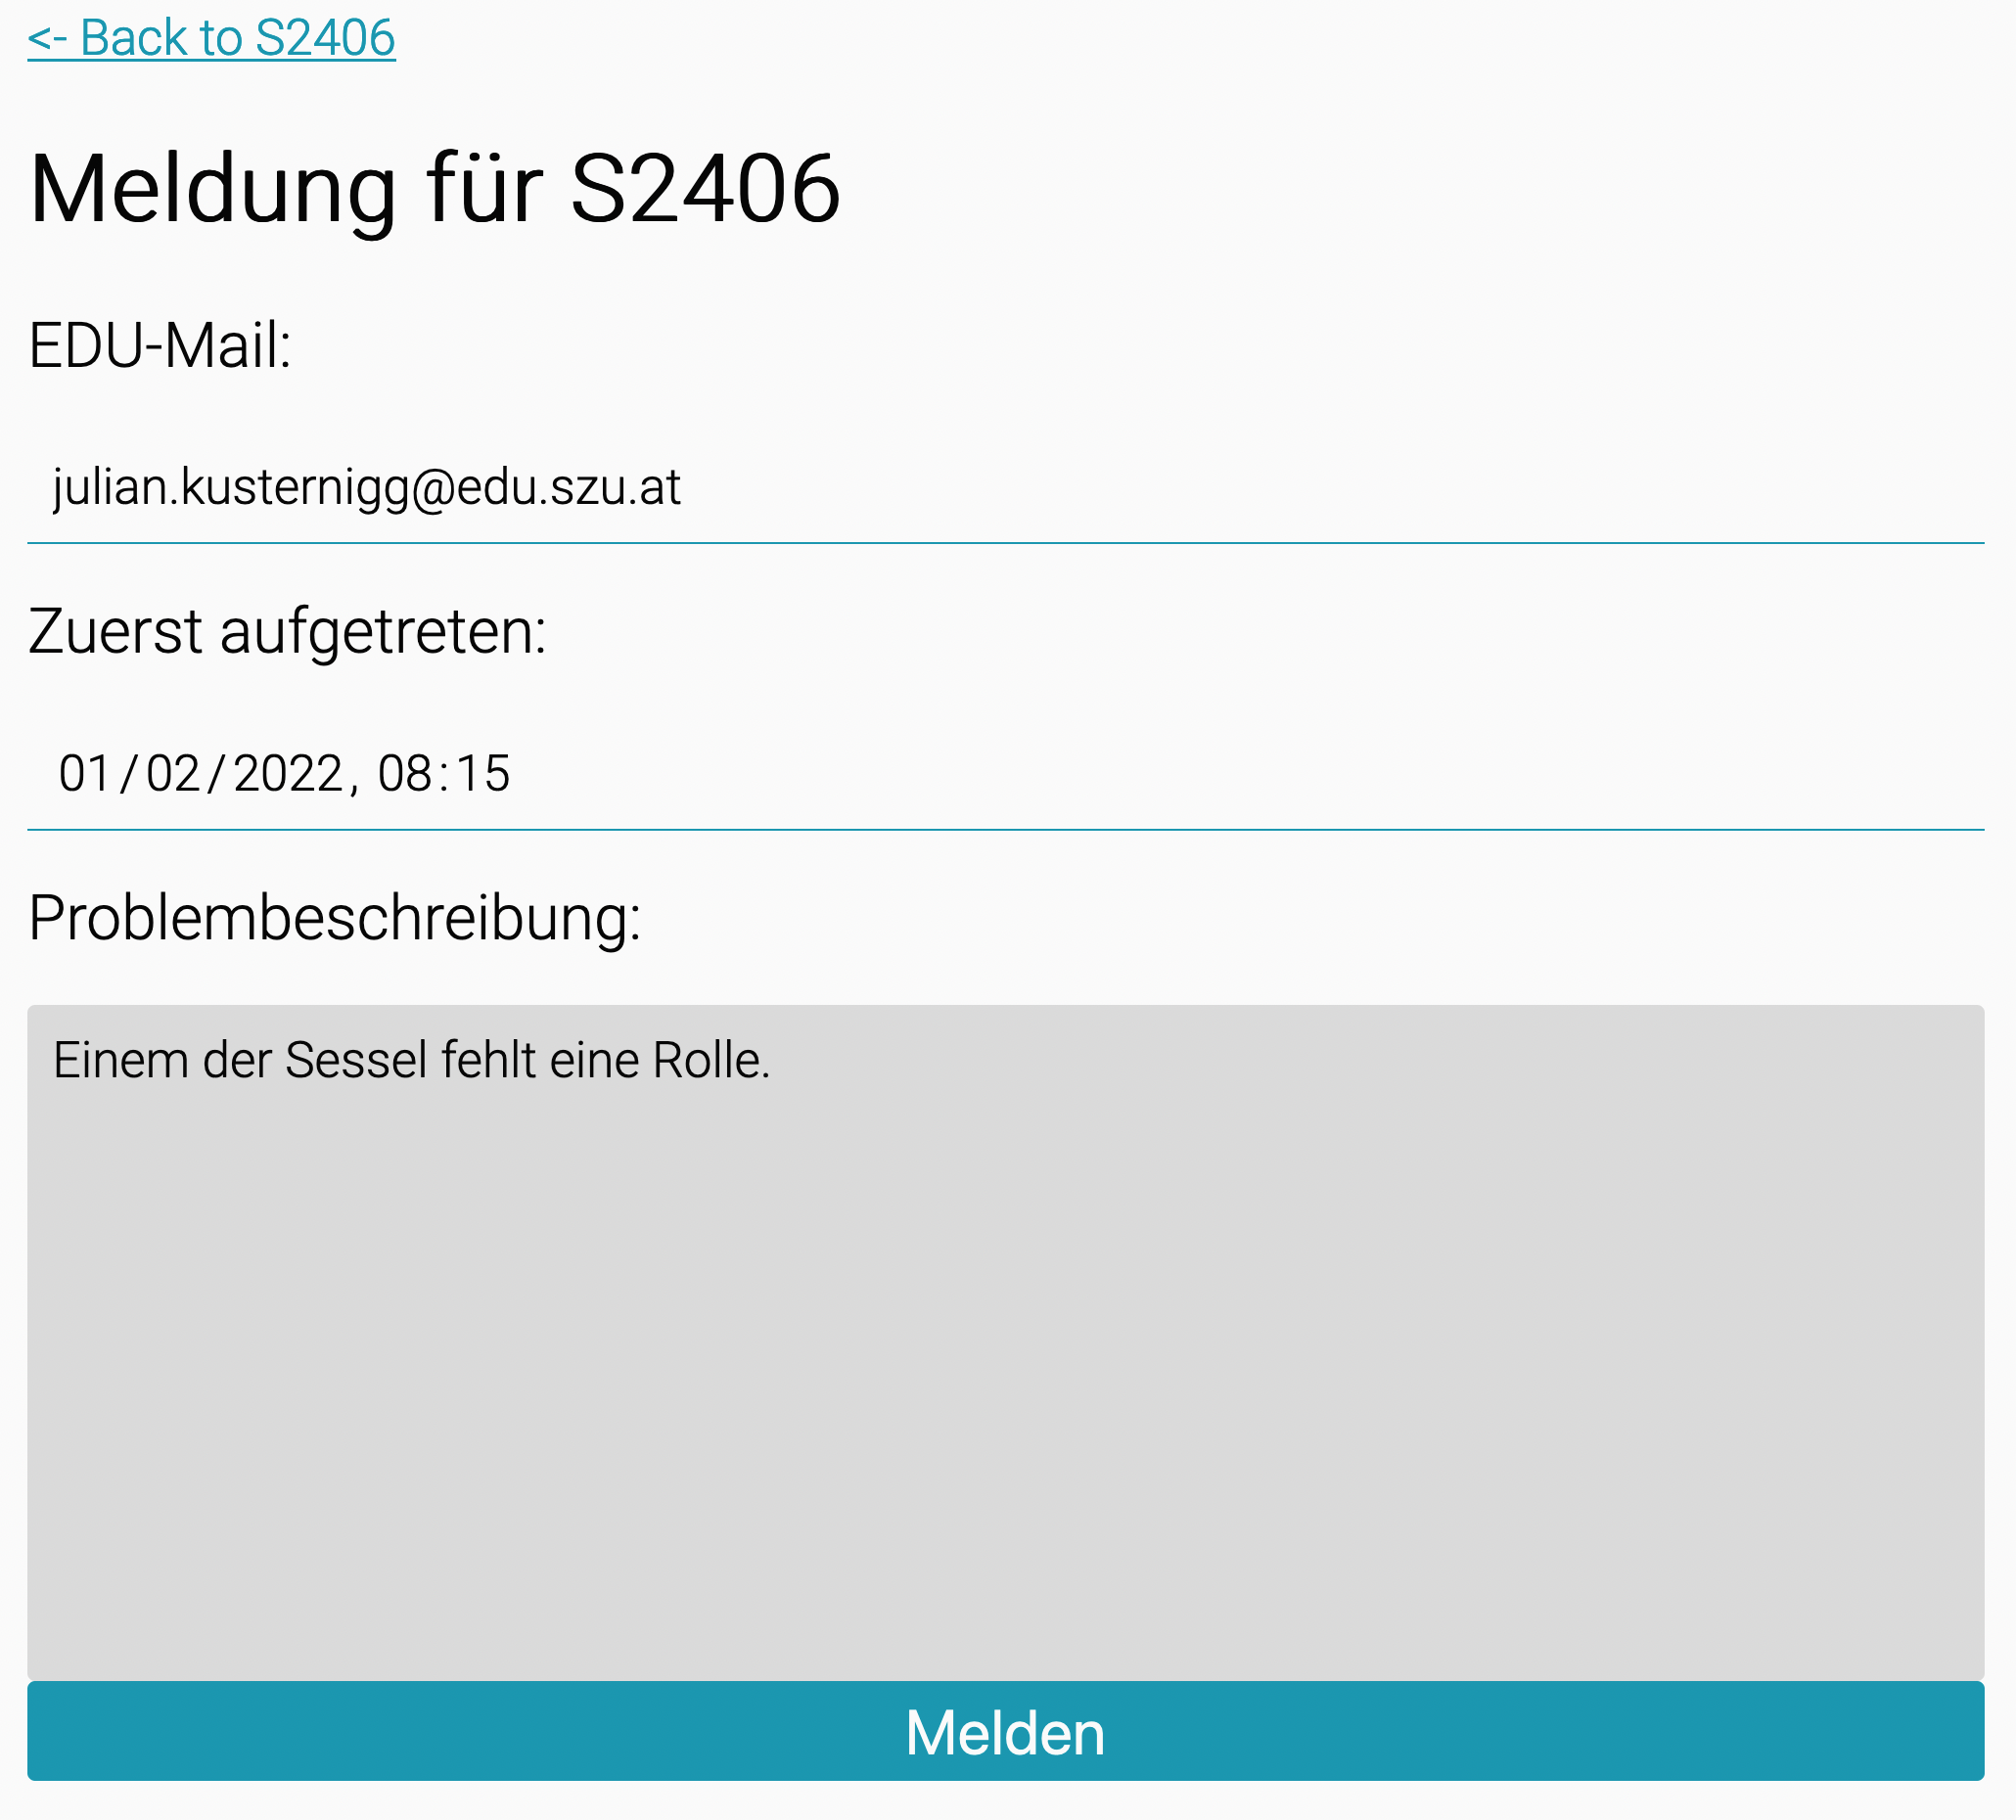
\includegraphics[width=120mm]{media/WebComponents/Meldungsseite_light.png}
    \caption{Meldungsseite}
\end{figure}

Eine Buchungsanfrage für einen Raum zu erstellen geht ebenso einfach, wie Defekte zu melden. Hierfür gibt man 3 Dinge an: Den Tag an dem man den Raum ausborgen will, die Unterrichtsstunde in der man startet und die Anzahl an Stunden die man den Raum nutzen möchte. Wie beim Melden, gibt man auch hier eine EDU-Mailadresse an und zusätzlich dazu sollte man noch einen Buchungsgrund angeben, um kurz zu schildern wofür man den Raum benötigt.

\begin{figure}[H]
    \centering
    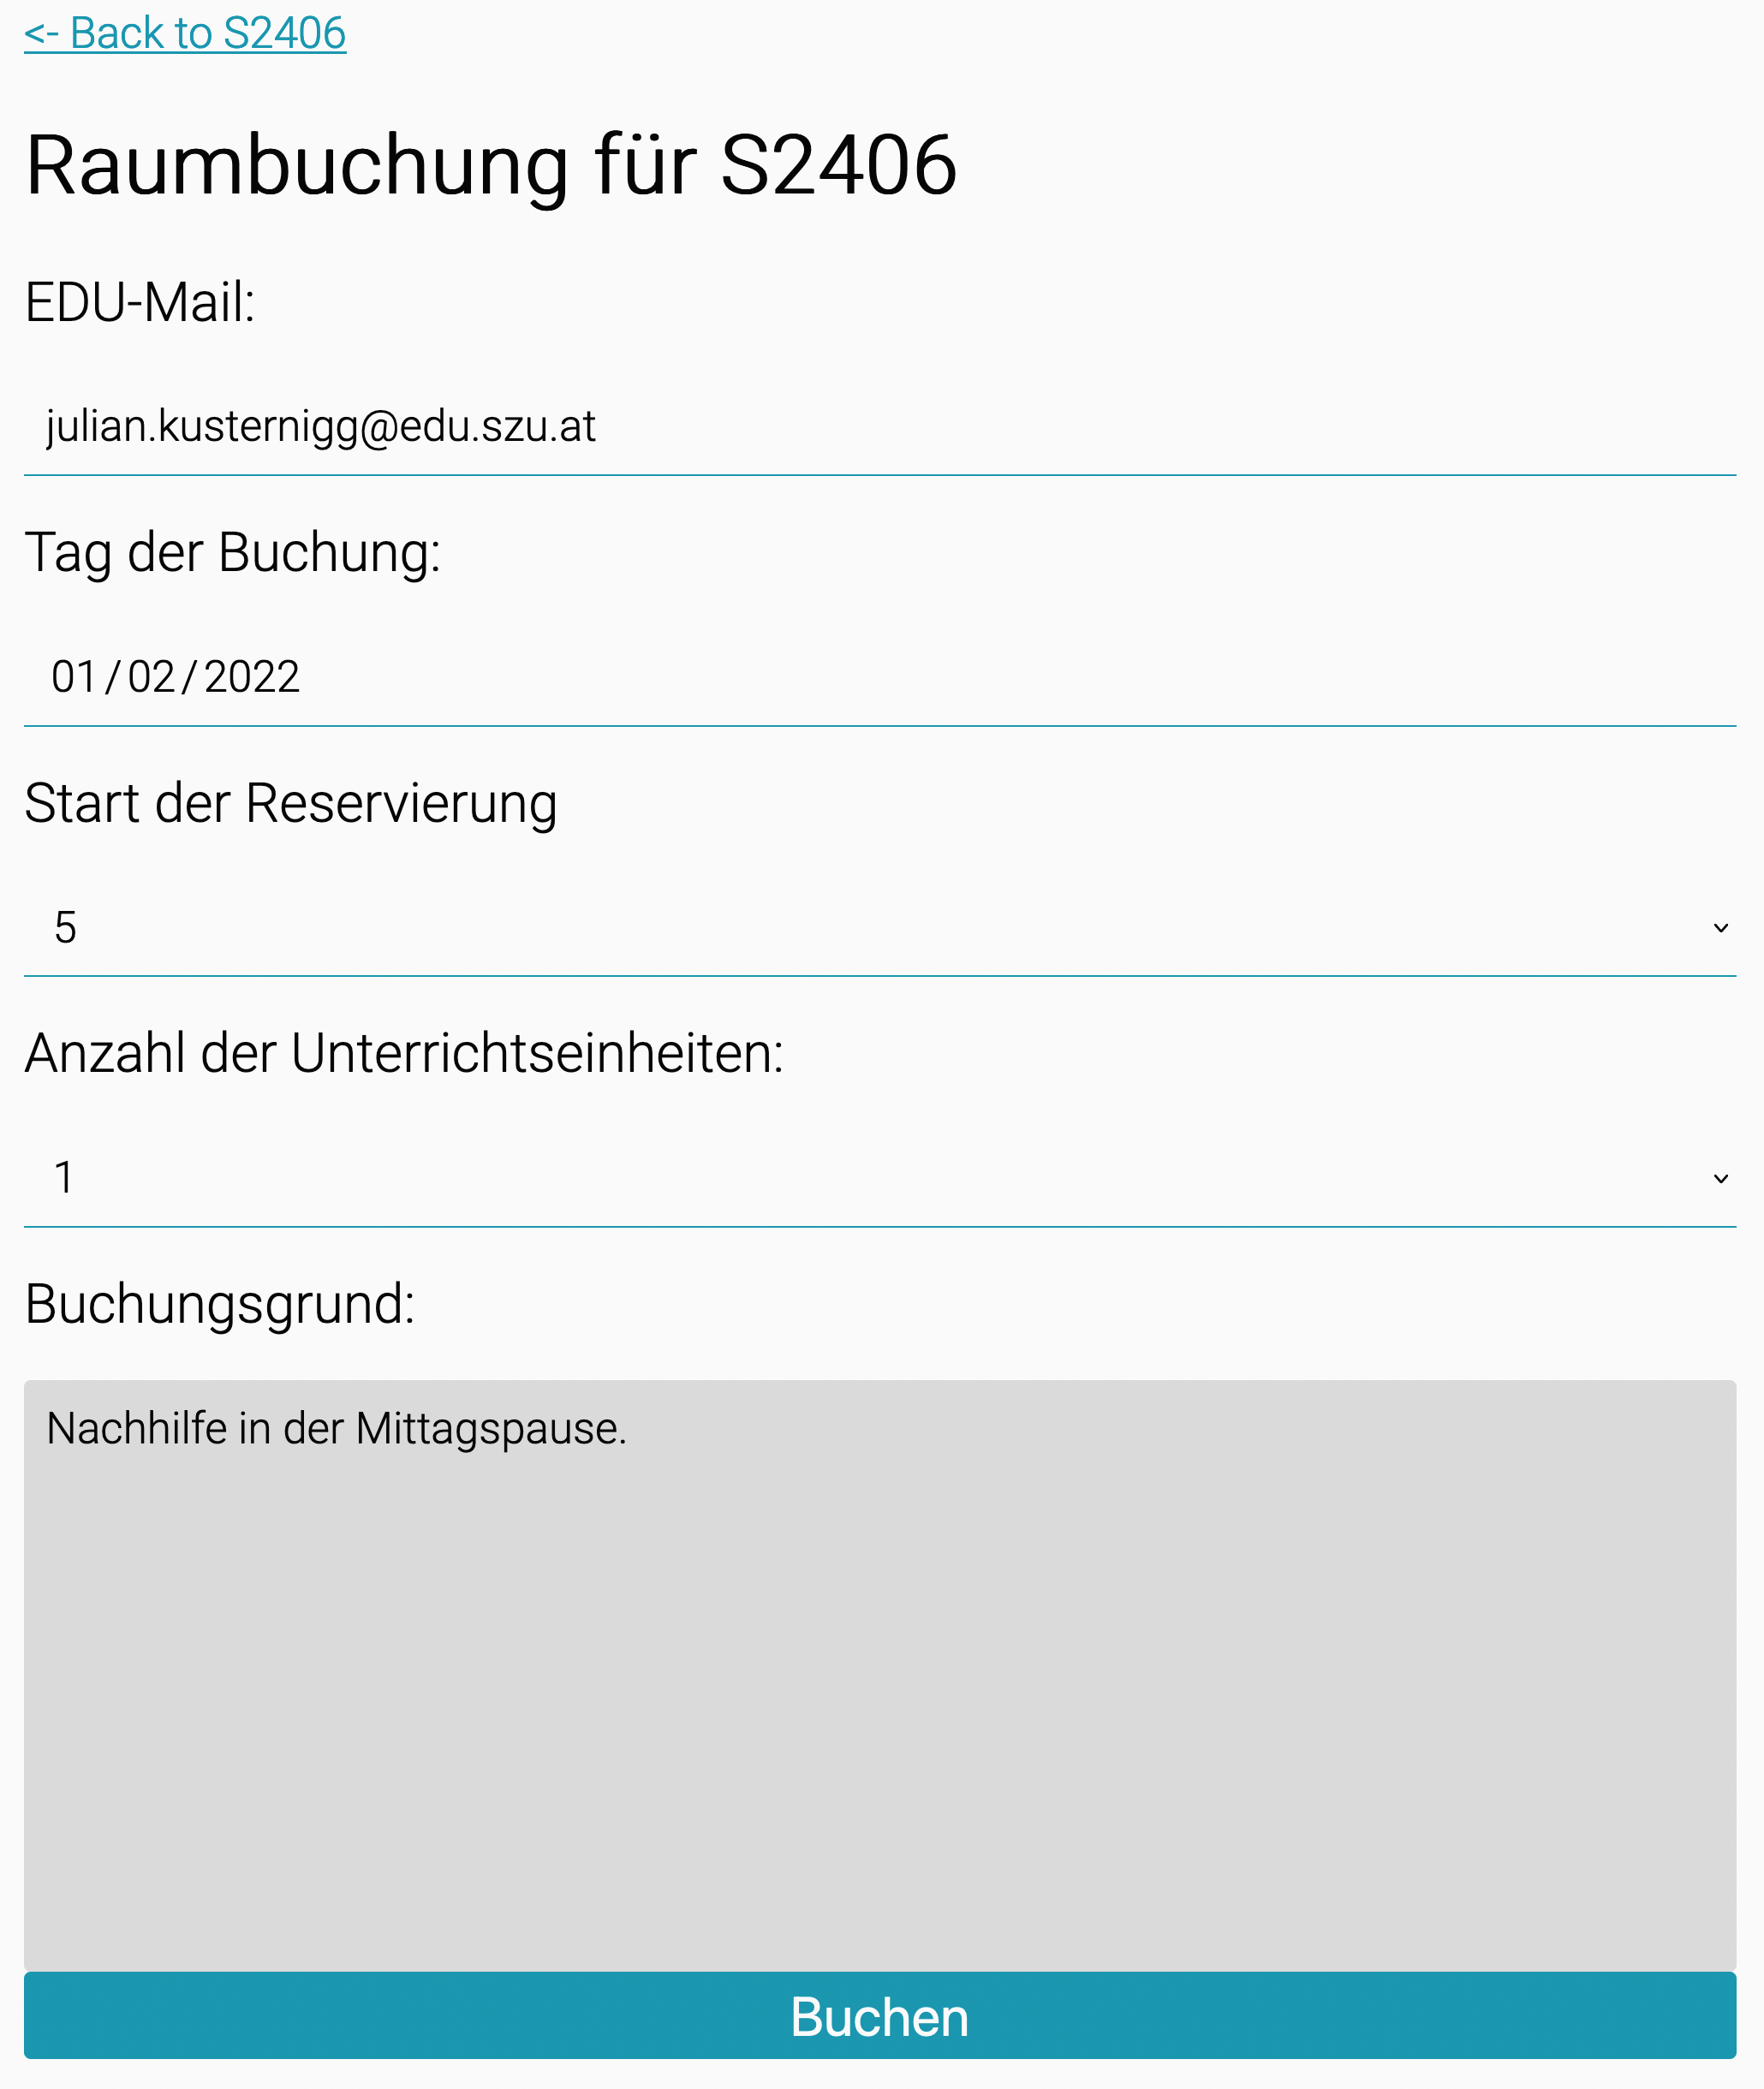
\includegraphics[width=120mm]{media/WebComponents/Buchungsseite_light.png}
    \caption{Meldungsseite}
\end{figure}


\hfive{"Admin Login" und "Dashboard"}

Um einen Überblick über Meldungen und Buchungen zu bekommen gibt es das "Admin Dashboard". Damit nicht jeder die Raumbuchungen und Defektmeldungen sieht, gibt es Administratorbenutzer mit denen man sich anmelden muss. Jede Buchung und Meldung ist einem Administratorbenutzer zugeteilt und kann somit von diesem abgearbeitet werden. Im Fall von ZELIA im Schulzentrum Ungargasse, sind Admins meist Abteilungsleiter*innen oder Lehrer*innen, die für den gemeldeten oder gebuchten Raum zuständig sind. 

Wie schon gesagt muss man angemeldet sein um Zugriff auf alle Meldungen und Buchungen zu haben. Hierfür gibt es die "Admin Login"-Seite, welche über den normalen ZELIA-Webserver aufgerufen werden kann. Auf dieser Webseite findet man eine Komponente die ein Anmeldeformular anzeigt. Wenn man sich anmeldet wird die Anfrage an den Server geschickt und auf die Antwort gewartet. Wenn der Server mit einem "JSON-Web-Token" (siehe Kapitel Authentifizierung "Json Web Token (JWT)") antwortet, wird dieser im "Sessionstorage" (siehe Kapitel "Webspeicher") gespeichert und man wird auf die Übersichtsseite weitergeleitet.

\begin{figure}[H]
    \centering
    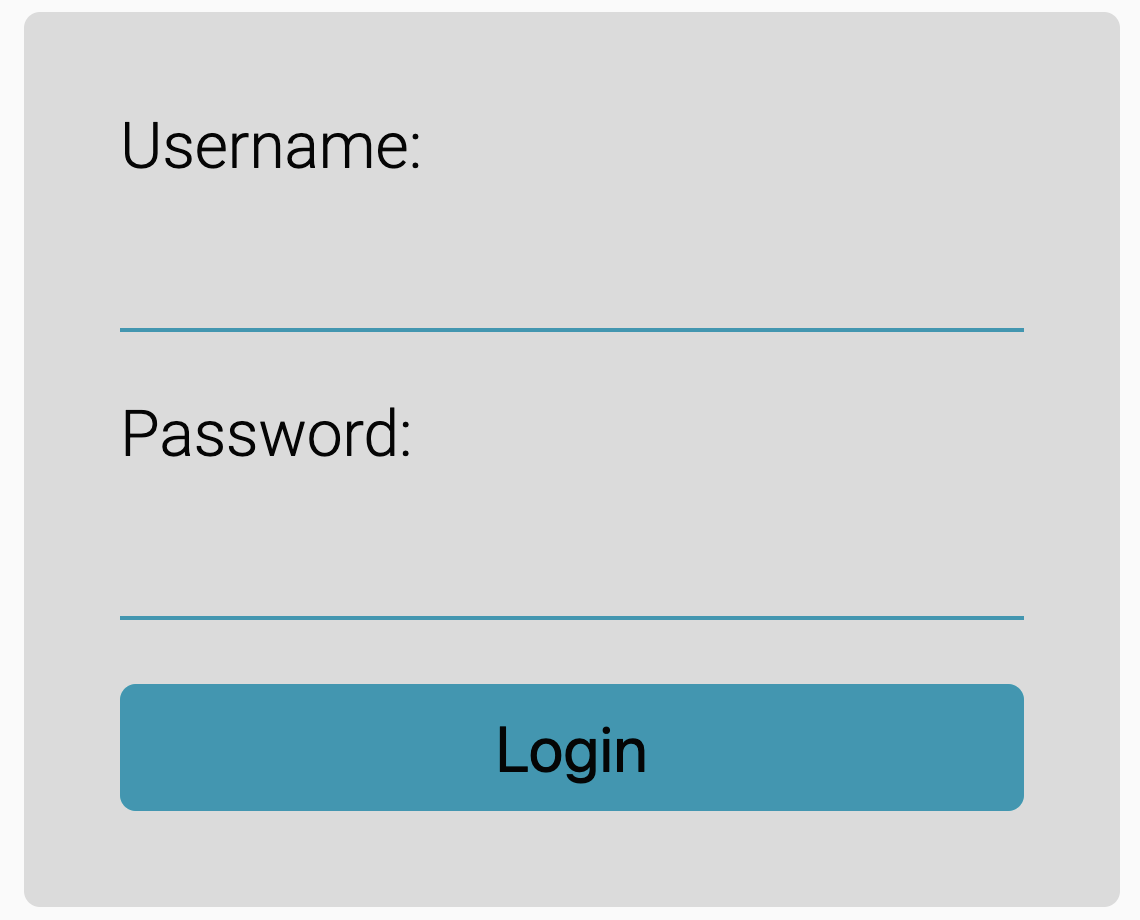
\includegraphics[width=120mm]{media/WebComponents/Login_light.png}
    \caption{Anmeldeseite}
\end{figure}

Landet man auf der "Admin Dashboard"-Seite wird zuerst überprüft ob ein Token im "Sessionstorage" gespeichert ist. Wenn Keiner vorhanden ist wird man sofort auf die Anmeldeseite umgeleitet. Bei einem vorhanden Token werden alle benötigten Request, die den Filtereinstellungen entsprechen, vom Server abgefragt. In dieser Anfrage wird auch der Token mitgeschickt. Am Server wird geprüft ob der Token gültig ist und wenn dies der Fall ist bekommt der Client die angefragten Daten. Ist der Token ungültig schickt der Server dem Client den HTTP-Code 401 "Unauthorized", woraufhin man auch auf die Anmeldeseite umgeleitet wird.

Hat der Client die Buchungen und Meldungen erhalten, verwendet es zwei Komponenten um diese Anzuzeigen. Anders als auf den anderen Seiten werden mehrere Instanzen dieser beiden Komponenten erstellt um alle Daten darzustellen. Jede Buchung und Meldung ist somit in einer eigenen Instanz einer Komponente untergebracht. Beide dieser Komponenten können aufgeklappt werden um alle damit verknüpften Informationen einzusehen. Zugeklappt bestehen sie aus einer Zusammenfassung der Daten. 

Die Buchungskomponente hat zwei verschiedene Knöpfe um die Buchungsanfrage zu verarbeiten. Einen zum "Akzeptieren" und den Anderen zum "Ablehenen". Zusätzlich könnte man noch einen kurzen Informationstext schreiben, der den Buchenden mit der Buchungsbestätigung per EDU-Mailadresse gesendet wird. 

Meldungen haben nur einen Knopf um den Status der Meldung auf "geschlossen" zu setzten. Im Hintergrund gäbe es mehrere Auswahlmöglichkeiten eines Status aber im Frontend ist noch nicht mehr implementiert, da wir uns darauf geinigt haben, dass es fürs erste nicht notwendig ist.

% TODO: Bild von Dashbord
TODO: Bild von Dashboard